\section{Laborfertiger Aufbau}

Der Laborfertige Aufbau wird auf Kugellagern gelagert, sowie mit einer Bremsscheibe gebremst, was ein wiederholtes Durchführen des Versuches ermöglicht, da die beim Bremsen erzuegte Hitze besser zerstreut wird.

In der Visualisierung nicht definiert sind:

\begin{itemize}
    \item Montage der Bremsbacken
    \item Montage der Wägezelle
    \item Montage des IR-Sensors
\end{itemize}

Falls die Laborversion wie geplant angefertigt wird, würde dies in etwa wie folgt aussehen.

\begin{figure}[H]
    \begin{center}
        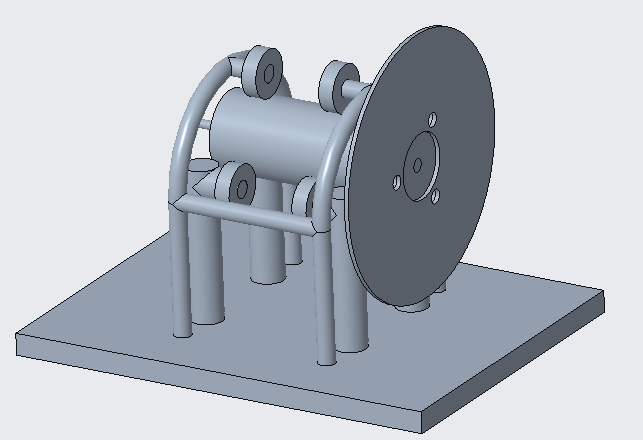
\includegraphics[width=0.3\textwidth]{versuchsaufbau2.PNG}
        \caption{3D Modell für den Laboraufbau}
    \end{center}
\end{figure}